\section{Derivatives for example functions}

\begin{figure}[h]
		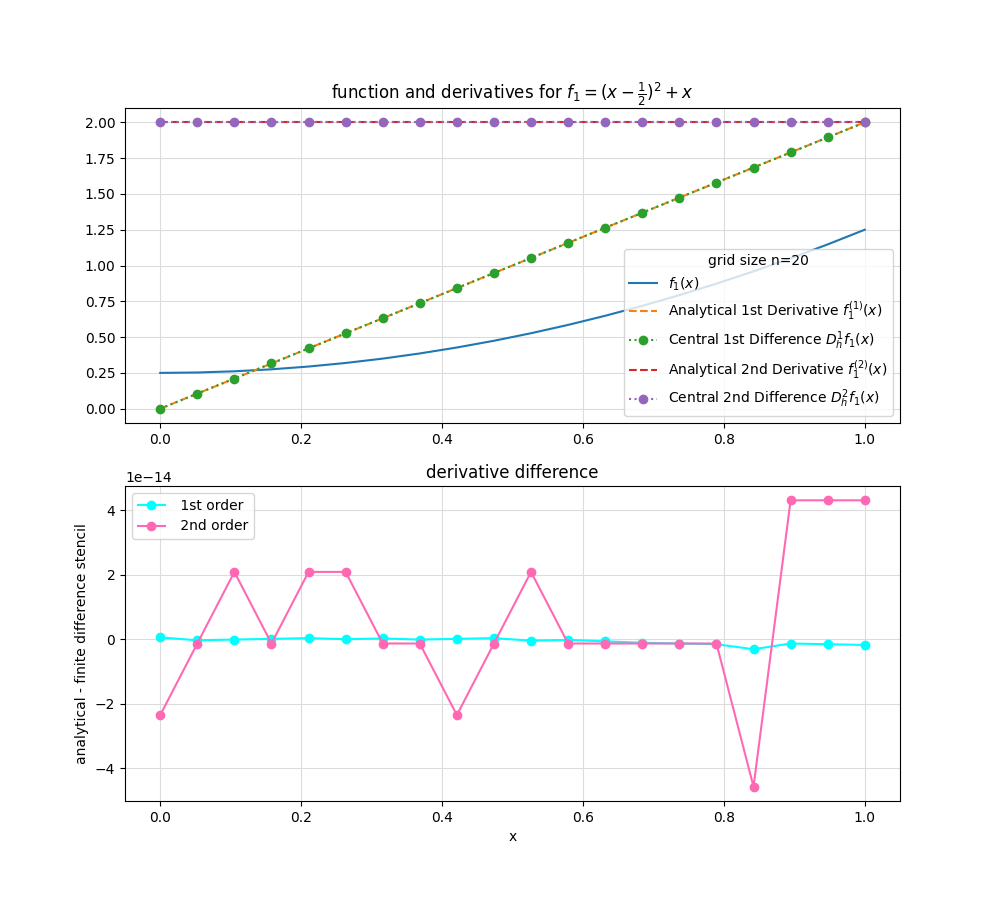
\includegraphics[scale=0.7]{plot_differences_analytical_finite_differences_f_1_n_20}
		\caption{Upper panel: Function $f_1$ in blue, dashed lines symbolize its analytical derivatives, dotted lines the finite difference approximation to the derivative. $n= 20$  Lower panel: The cyan and pink lines show the difference between analytical and numerically generated derivatives.}
\end{figure}

\begin{figure}
		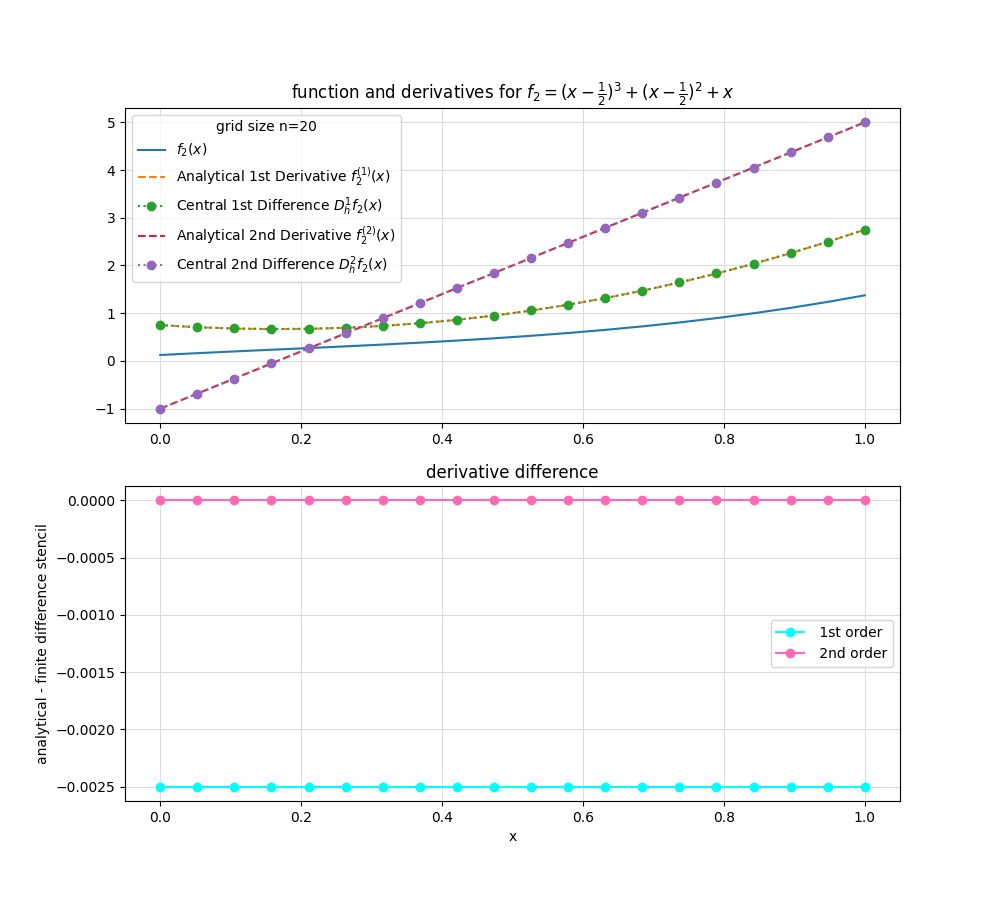
\includegraphics[scale=0.7]{plot_differences_analytical_finite_differences_f_2_n_20}
		\caption{}
\end{figure}

\begin{figure}
		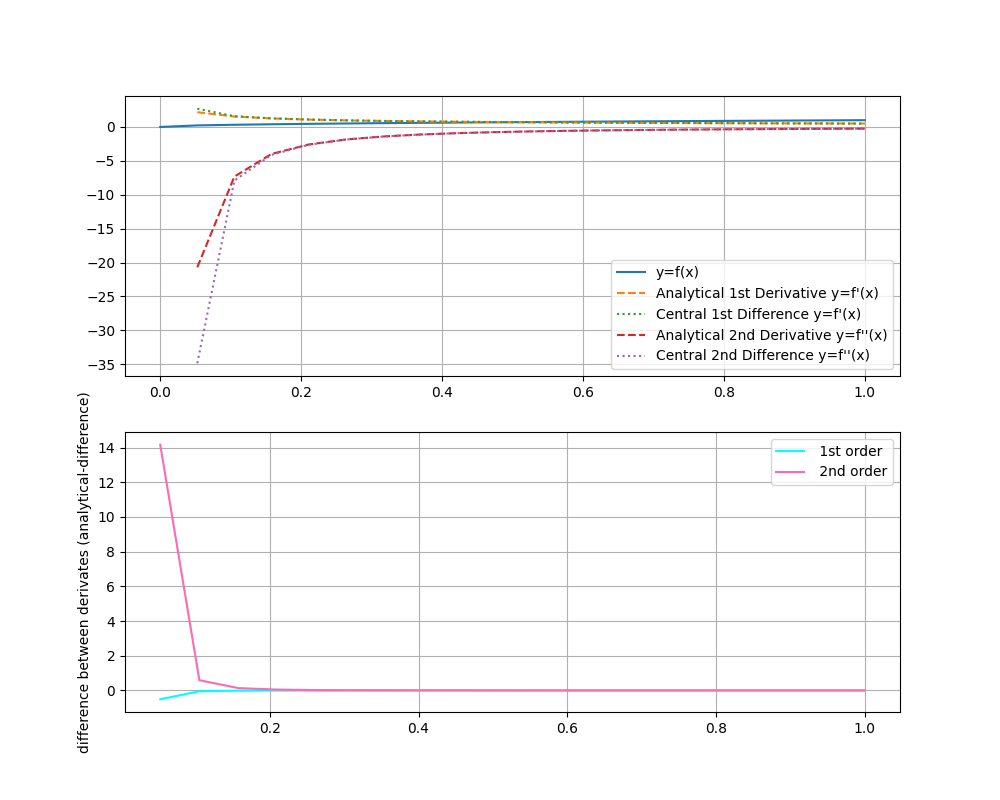
\includegraphics[scale=0.7]{plot_differences_analytical_finite_differences_f_3_n_20}
	\caption{}
\end{figure}

\begin{figure}
		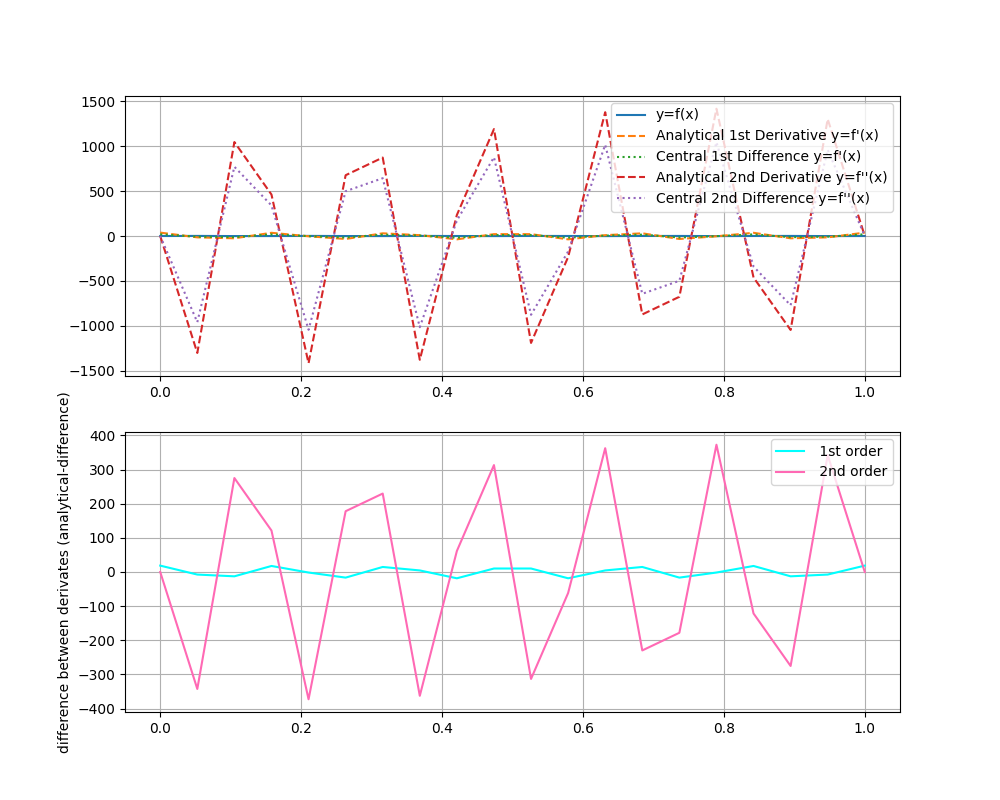
\includegraphics[scale=0.7]{plot_differences_analytical_finite_differences_f_4_n_20}
		\caption{}
\end{figure}


\begin{figure}
		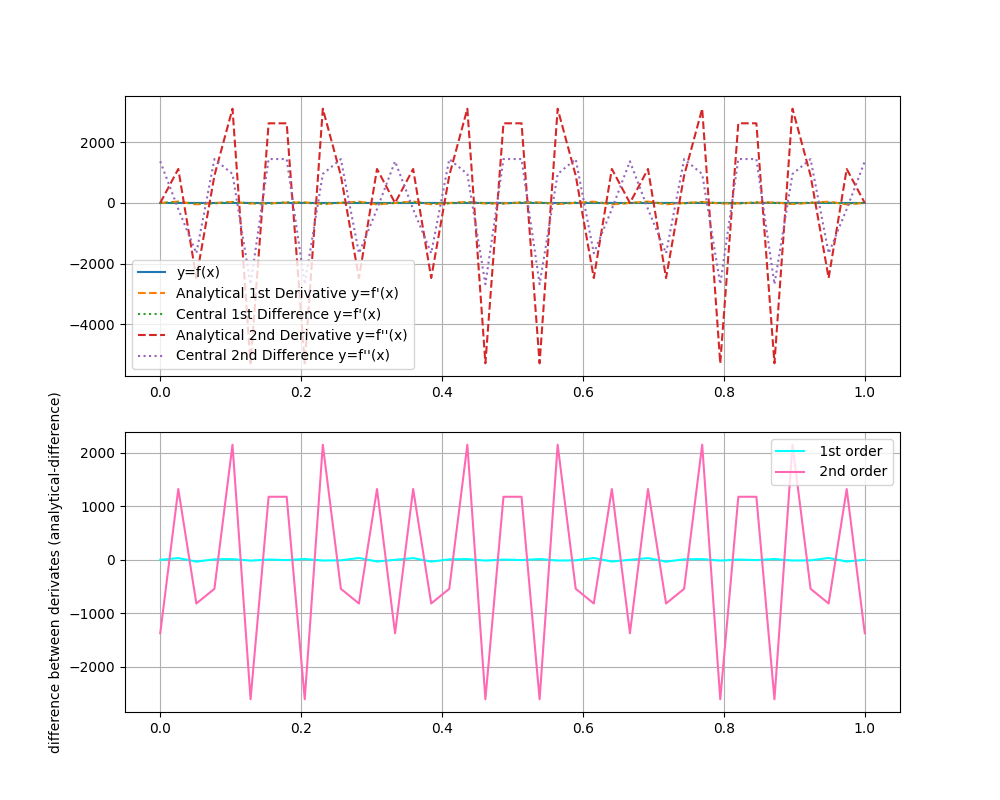
\includegraphics[scale=0.7]{plot_differences_analytical_finite_differences_f_5_n_40}
		\caption{}
\end{figure}


\begin{figure}
		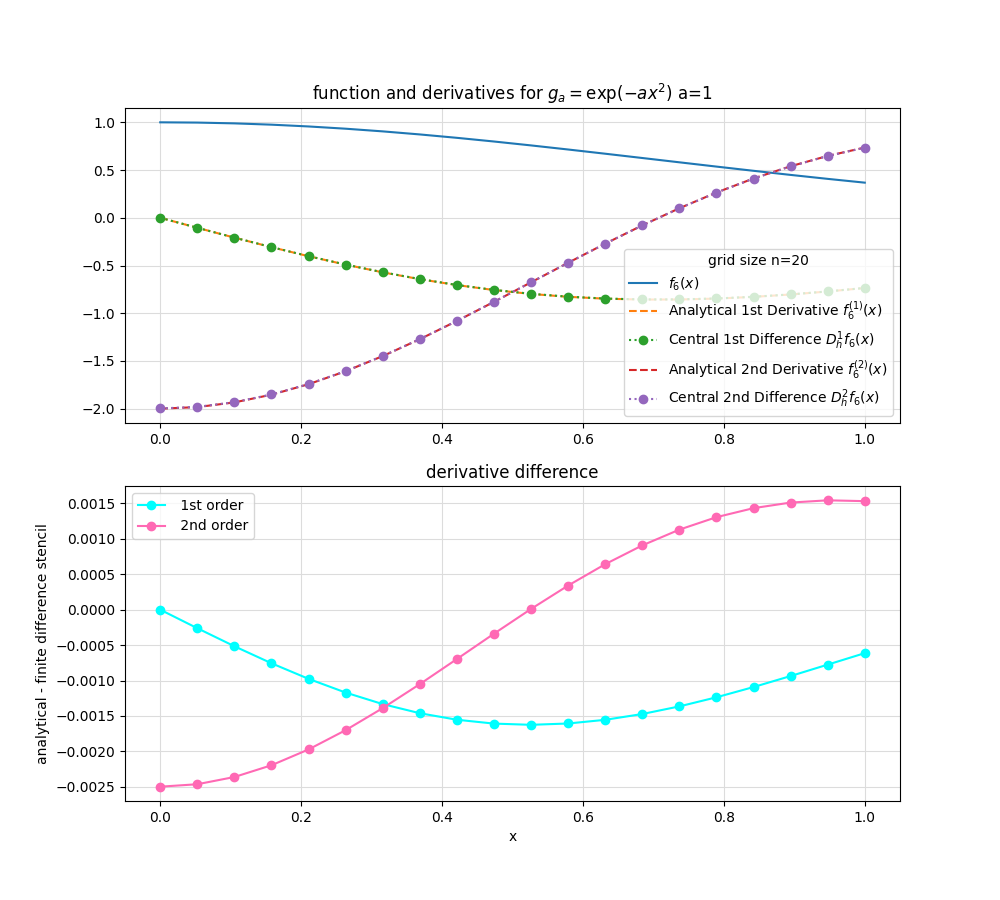
\includegraphics[scale=0.7]{plot_differences_analytical_finite_differences_f_a_n_20_a_1}
		\caption{}
\end{figure}

\newpage